\documentclass[a4paper,10pt]{article}
\usepackage[utf8]{inputenc}
\usepackage[english] {babel}
\usepackage[T1]{fontenc}
\usepackage{lmodern}
\usepackage{graphicx}
\usepackage{graphics}
\usepackage{ulem}
\usepackage{amssymb}
\usepackage{url}
\usepackage[a4paper]{geometry}
\geometry{hscale=0.7,vscale=0.7,centering}
\usepackage{vmargin}
\usepackage{amsmath}
\usepackage{amssymb}
\usepackage{amsthm}
\usepackage{moreverb}
\usepackage{listings}
\usepackage{enumerate}
%\usepackage{enumitem}
\newtheorem{theorem}{Théorème}[section]
\newtheorem{defi}{Définition}[section] 
\newtheorem{prop}{Propriété}[section] 
\usepackage{color}
\definecolor{gris}{rgb}{0.95,0.95,0.95}
\lstset{numbers=left, tabsize=4, backgroundcolor=\color{gris},
frame=single, breaklines=true,
keywordstyle=\color{black},
stringstyle=\ttfamily,
framexleftmargin=6mm, xleftmargin=6mm}
%opening
\title{LINGI 2261 : Artificial Intelligence \\
Assignement 3 - Mid-Project}
\author{Rochet Florentin - Debroux Léonard} 
\date{Année académique 2011-2012}

\begin{document}

	\begin{titlepage}
		\begin{center}
			{\huge LINGI2261: Artificial Intelligence}\\
			\vspace{0.4cm}
			
			{\Large {Professor : Yves Deville\\ \vspace{0.2cm} Teaching assistants : Cyrille Dejemeppe and Jean-Baptiste Mairy  }}\\
			\vspace{0.6cm}
			
			{\Large \textit{Assignment 4 : Local Search and Propositional Logic}}\\
			\vspace{1.2cm}

			\texttt{}\\
			\vspace{0.2cm}

			
\includegraphics[height=10cm]{pageGarde.png}\\
			\vspace{0.1cm}
			{\Large \textbf{Universit\'e Catholique de Louvain}}
			\vspace{0.7cm}

			Groupe 37 \\
			\vspace{0.2cm}
			
			Florentin Rochet \\
			Léonard Debroux\\
			\vspace{0.2cm}
			2012-2013\\
		\end{center}
	\end{titlepage}

	\newpage
	
\section{The Traveling Salesman Problem}
\subsection{Diversification versus Intensification}
\subsubsection{Question 1}
The point is to find a solution that is as good as possible, while avoiding the bad complexity of the exact solution of the TSP. 
We'll formulate each state as a list of ordered cities and a variable containing the sum of the cost of the distances between two adjacent cities in the list.\\
A solution will be a tuple containing the list of cities, which order follows the indexes in the list, and a double containing the total cost of the solution).\\
The successor function will take an admissible path for the tsp and yield all the possible swaps of two cities in the list.\\
Symmetrical states will be avoided by considering that the swaps of two cities $(c1, c2)$ and $(c2, c1)$ are the same.\\
As said before, the evaluation function sums the distance between each couple of $p_{i}, p_{i+1}$ in the list to give the total cost of the solution.
The distances are recovered from the distance matrix given in the input file.
\subsubsection{Question 2}
The implementation of the tree different strategies are in the python modules: \verb@randomwalk.py@, \verb@maxvalue.py@ and \verb@randomized_maxvalue.py@.
\subsubsection{Question 3}
%\begin{itemize}[noitemsep,nolistsep]
\begin{itemize}
\itemsep0em
\item Algo1 stands for randomwalk.py
\item Algo2 stands for maxvalue.py
\item Algo3 stands for randomzied\_maxvalue.py \\
\end{itemize}
\begin{center}
\begin{tabular}{|c|c|c|c|}
\hline 
att48.tsp & Algo1 & Algo2 & Algo3 \\ 
\hline 
Comp time [s] & 0.45 & 2.76 & 3.035 \\ 
\hline 
Best sol. & 125431.15 & 41881 & 40692.82 \\ 
\hline 
\# Steps & 34.6 & 28 & 96.2 \\ 
\hline 
\end{tabular} 
\end{center}
\begin{center}
\begin{tabular}{|c|c|c|c|}
\hline 
bayg29.tsp & Algo1 & Algo2 & Algo3 \\ 
\hline 
Comp time [s] & 0.141 & 0.64 & 0.666 \\ 
\hline 
Best sol. & 21870.78 & 9003.8 & 9848.76 \\ 
\hline 
\# Steps & 28.6 & 30 & 76.4 \\ 
\hline 
\end{tabular} 
\end{center}
\begin{center}
\begin{tabular}{|c|c|c|c|}
\hline 
bays29.tsp & Algo1 & Algo2 & Algo3 \\ 
\hline 
Comp time [s] & 0.145 & 0.63 & 0.687 \\ 
\hline 
Best sol. & 22064.32 & 9003.8 & 10786.66 \\ 
\hline 
\# Steps & 43.4 & 30 & 65 \\ 
\hline 
\end{tabular} 
\end{center}
\begin{center}
\begin{tabular}{|c|c|c|c|}
\hline 
berlin52.tsp & Algo1 & Algo2 & Algo3 \\ 
\hline 
Comp time [s] & 0.546 & 3.45 & 3.73 \\ 
\hline 
Best sol. & 23485.24 & 10075.2 & 9681.88 \\ 
\hline 
\# Steps & 61 & 21 & 92.6 \\ 
\hline 
\end{tabular} 
\end{center}
\begin{center}
\begin{tabular}{|c|c|c|c|}
\hline 
dantzig42.tsp & Algo1 & Algo2 & Algo3 \\ 
\hline 
Comp time [s] & 0.327 & 1.85 & 1.97 \\ 
\hline 
Best sol. & 912.24 & 650.1 & 712.72 \\ 
\hline 
\# Steps & 44.2 & 17 & 73 \\ 
\hline 
\end{tabular} 
\end{center}

\subsubsection{Question 4}
\begin{center}
\begin{figure}[!ht]
		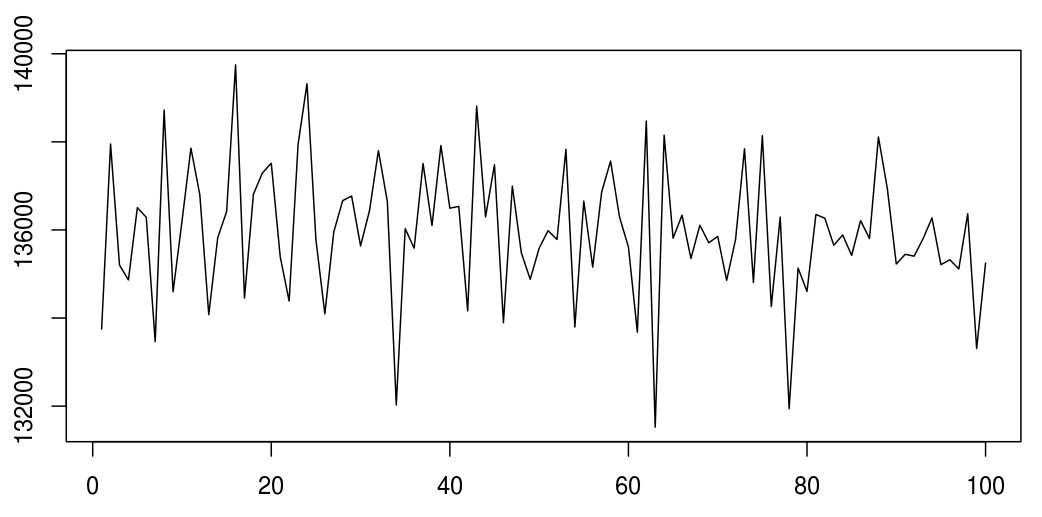
\includegraphics[scale=.4]{randomwalk.png}
	\caption{randomwalk.py}
\end{figure}
\end{center}
\begin{center}
\begin{figure}[!ht]
		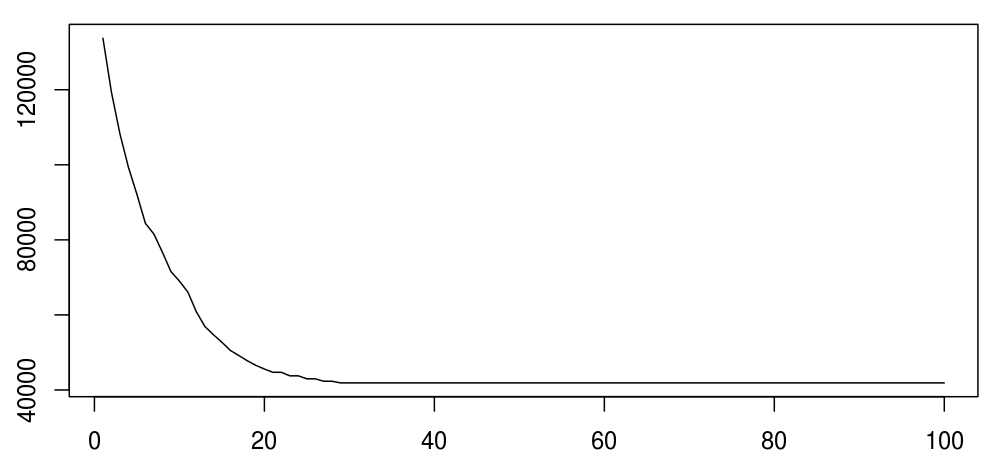
\includegraphics[scale=.4]{maxvalue.png}
	\caption{maxvalue.py}
\end{figure}
\end{center}
\begin{center}
\begin{figure}[!ht]
		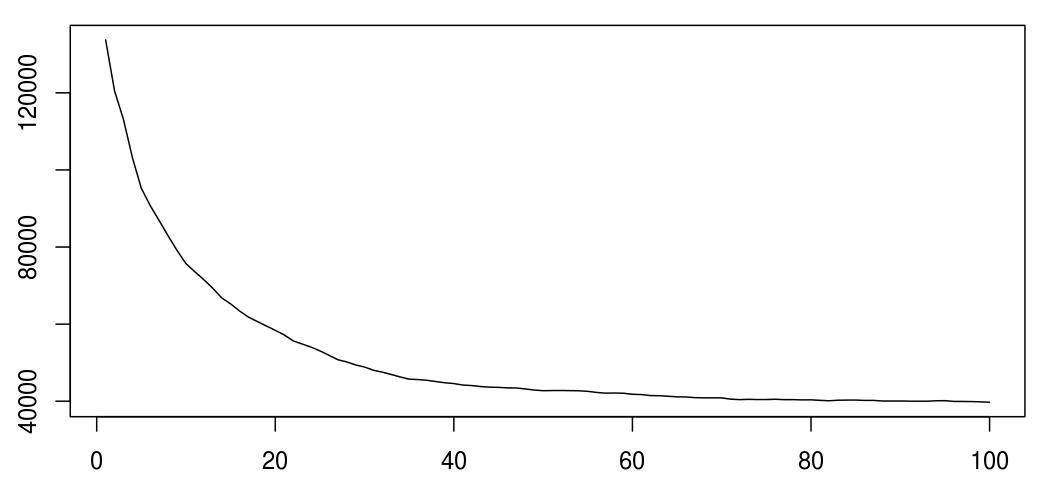
\includegraphics[scale=.4]{randomized_maxvalue.png}
	\caption{randomized\_maxvalue.py}
\end{figure}
\end{center}
When randomness was part of the algorithms, there were 5 tests for each one (like we did for the third question).

\subsubsection{Question 5}
	\begin{enumerate}[(a)]
		\item \textit{maxvalue} and r\texttt{andomized\_maxvalue both} seem to work well. There no real winner between those two.
		\item Well because our tests show that two strategies are quite good, the only suitable reason for them to beat \texttt{randomwalk} is that it does not look for a best path when choosing a step.
		\item The limitation of \texttt{randomwalk} is that it does not look for a good path, so there is less chance to find the best one.\\
		Concerning \texttt{maxvalue}, it might fall into a local optimum {\Huge and have difficulties to go out of it.}\\
		\texttt{randomized\_maxvalue} should be the best as it can easily avoid local optima and so, have a chance to find the global one.
		\item {\Huge ASK FLO}
		\item There must be a trade off between intensification and diversification because intensification ensures that we go for a good solution, while diversification ensures that we explore several possibilities. \\
		Intensification alone (\verb@maxvalue.py@) would cause the solution to find a local optimum without considering others paths to better solutions and diversification alone (\verb@randomwalk.py@) would cause to explore other paths but no necessarily the good ones.
	\end{enumerate}

\subsection{Some well-known strategies}
\subsubsection{Question 1}
\subsubsection{Question 2}
\subsubsection{Question 3}
\subsubsection{Question 4}
\subsubsection{Question 5}
\subsubsection{Question 6}



	
\newpage
	
	
	

\section{Propositional logic}
\subsection*{Models and logical connectives}

\subsubsection*{Question 1 : For each sentence, give the number of models that satisfy it (considering the
whole vocabulary).\\}

Since we are using Propositional logic, each variable can be either True or False. Therefore, for each sentences, we have as the number of possibles combinaisons the value 2 power the number of different variables in the sentence. The number of models will be the number of combinaisons which are making the sentence true. \\
This is shown in the following tabulars. \\

\begin {enumerate}
 \item $\beta : (A \vee B) \wedge(B \vee C)$
 \begin{center}

 \begin{tabular}{|c|c|c|c|c||c|}
	\hline
	A & B & C & $A \vee B$ & $B \vee C$& $\beta$ \\
	\hline 
	F & F & F & F & F & F \\
	\hline
	V & V & V & V & V & V \\
	\hline
	F & V & V & V & V & V \\
	\hline
	F & F & V & F & V & F \\
	\hline
	F & V & F & V & V & V \\
	\hline
	V & F & F & V & F & F \\
	\hline
	V & F & V & V & V & V \\
	\hline
	V & V & F & V & V & V \\
 	\hline
 \end{tabular}
 
 \end{center}
 Here we have 5 interpretations which are model of $\beta$
 \item $\beta : A \wedge B$\\
 
 \begin{center}

 \begin{tabular}{|c|c||c|}
	\hline
	A & B & $\beta$ \\
	\hline 
	F & F & F  \\
	\hline
	V & V & V  \\
	\hline
	F & V & F \\
	\hline
	V & F & F \\
	\hline
 \end{tabular}
  
 \end{center}
 
 Here we have 1 interpretation which is model of $\beta$
\item $\beta : (A \Rightarrow B) \Leftrightarrow C $


 \begin{center}

 \begin{tabular}{|c|c|c|c||c|}
	\hline
	A & B & C & $A \rightarrow B$ & $\beta$ \\
	\hline 
	F & F & F & V & F \\
	\hline
	V & V & V & V & V \\
	\hline
	F & V & V & V & V \\
	\hline
	F & F & V & V & V  \\
	\hline
	F & V & F & V & F \\
	\hline
	V & F & F & F & V \\
	\hline
	V & F & V & F & F \\
	\hline
	V & V & F & V & F \\
 	\hline
 \end{tabular}
  
 \end{center}
 Here we have 4 interpretations which are model of $\beta$
\end {enumerate}
\subsubsection*{Question 2 : Give two valid interpretations of the following sentence: $\beta : (A \wedge B) \Rightarrow C$ .}
Two valid interpretation for \beta are :
\begin{tabular}{|c|c|c|}
  \hline

\end{tabular}
\end{document}
